\section{Konfiguration und Bauen des Systems}
\label{cha:ver:sec:Konfiguration_und bauen_system}

In diesem Abschnitt werden vor allem die Werkzeuge erläutert, die zur Erstellung einer angepassten Linux-Distribution benötigt werden, sowie die Methode, mit der eine solche Distribution erstellt wird. Dabei wird ein Überblick über das Yocto-Projekt als Grundlage für die PetaLinux-Werkzeuge gegeben. Der Prozess der Erstellung einer Linux-Distribution mit den PetaLinux-Tools wird beschrieben. Darüber hinaus wird der Prozess der Konfiguration und Erstellung des Kernels und des Root-Dateisystems für den Zynq UltraScale+ MPSoC im Detail erklärt. \\
Um den PetaLinux-Build Prozess zu verstehen, ist es wichtig, bestimmte Schlüsselkonzepte im Zusammenhang mit dem Yocto-Projekt zu verstehen, darum wird in dem nächsten Abschnitt erst das Yocto-Projekt vorgestellt. 

\subsection{Das Yocto Projekt}

Die Arbeit mit dem Yocto-Projekt ist die Basis für die Erstellung einer Linux-Distribution mit den PetaLinux-Tools. Die PetaLinux-Tools nutzen den Build-Prozess des Yocto-Projekts zur Erstellung der Linux-Distribution und verbergen damit die Komplexität, die mit der direkten Verwendung des Yocto-Projekts einhergeht. Sie bieten eine einfach zu bedienende Kommandozeilenschnittstelle, die es Entwicklern erleichtert, das Betriebssystem zu erstellen. \\
Das Yocto-Projekt jedoch  ist ein Open-Source-Projekt, das auch Entwicklern hilft, angepasste Linux-Distributionen für ihre eingebetteten Systeme zu erstellen, die verschiedene Prozessorarchitekturen unterstützen. Um die Distribution zu erstellen, verfügt das Projekt über eine Sammlung von Werkzeugen und Mechanismen zur Erstellung von angepassten Komponenten wie FSBL, U-Boot, Device-Tree und Kernel-Image zum Booten von Linux auf Embedded-Systemen.\\
Das Yocto-Projekt verwendet ein Schichtenmodell(Layer Model), das den Benutzern die Flexibilität bietet, schichtspezifische Änderungen vorzunehmen. 

\subsubsection{Yocto Layer}

Yocto-Layer oder Meta-Daten-Layer sind Repositories von Konfigurations- und Build-Skripten zusammen mit Build-Spezifikationen (BitBake-Rezepten), die dem Yocto-Build-System (OpenEmbedded Build System) mitteilen, wie eine angepasste Linux-Distribution zu bauen ist. Sie können hardwarespezifisch sein, oder so flexibel sein, dass sie auch für andere Architekturen angepasst werden können
Je nachdem, wie komplex der Entwickler eine bestimmte Schicht gestalten möchte, können Layer verwendet werden, um bestimmte Build-Aufgaben zu trennen oder zu kombinieren. Die Erhöhung der Build-Aufgaben, die mit  bestimmten Layers verbunden sind, erhöht die Komplexität des Projekts und erschwert den Entwicklern die Anpassung, Wartung und Wiederverwendung von diesen Layers. 

%or \small or \footnotesize etc.
\begin{lstlisting}[backgroundcolor = \color{lightgray},basicstyle=\scriptsize\ttfamily,caption={Inhalt einer bblayers.conf Datei in Yocto},label=lst:bblayers,language=bash,framexleftmargin = 2em]
	LCONF_VERSION = "7"
	
	BBPATH = "${TOPDIR}"
	SDKBASEMETAPATH = "/home/landry/mein_Abschluss/IPU-NG/components/yocto"
	BBLAYERS := " \
	${SDKBASEMETAPATH}/layers/core/meta \
	${SDKBASEMETAPATH}/layers/core/meta-poky \
	${SDKBASEMETAPATH}/layers/meta-openembedded/meta-perl \
	${SDKBASEMETAPATH}/layers/meta-openembedded/meta-python \
	${SDKBASEMETAPATH}/layers/meta-openembedded/meta-filesystems \
	${SDKBASEMETAPATH}/layers/meta-openembedded/meta-gnome \
	${SDKBASEMETAPATH}/layers/meta-openembedded/meta-multimedia \
	${SDKBASEMETAPATH}/layers/meta-openembedded/meta-networking \
	${SDKBASEMETAPATH}/layers/meta-openembedded/meta-webserver \
	${SDKBASEMETAPATH}/layers/meta-openembedded/meta-xfce \
	${SDKBASEMETAPATH}/layers/meta-openembedded/meta-initramfs \
	${SDKBASEMETAPATH}/layers/meta-openembedded/meta-oe \
	${SDKBASEMETAPATH}/layers/meta-xilinx/meta-xilinx-bsp \
	${SDKBASEMETAPATH}/layers/meta-xilinx/meta-xilinx-pynq \
	${SDKBASEMETAPATH}/layers/meta-xilinx/meta-xilinx-contrib \
	${SDKBASEMETAPATH}/layers/meta-xilinx/meta-xilinx-standalone \
	${SDKBASEMETAPATH}/layers/meta-xilinx-tools \
	${SDKBASEMETAPATH}/layers/meta-petalinux \
	${SDKBASEMETAPATH}/layers/meta-som \
	${SDKBASEMETAPATH}/layers/meta-security \
	${SDKBASEMETAPATH}/layers/meta-security/meta-tpm \
	/home/landry/mein_Abschluss/IPU-NG/project-spec/meta-user \
	/home/landry/mein_Abschluss/IPU-NG/components/yocto/workspace \
	/home/landry/mein_Abschluss/IPU-NG/project-spec/meta-ipu_ng \
	"
\end{lstlisting}


\subsubsection{Poky}
Bei Poky handelt es sich um eine Referenzdistribution, die vom Yocto-Projekt verwendet wird, um eigene Linux-Distributionen zu erstellen. Sie besteht aus dem OpenEmbedded Build-System und den Metadaten, die dem Build-System helfen, eine minimale Linux-Distribution zu erstellen. Die minimale Linux-Distribution, die mit Poky erstellt wurde, wird mit weiteren Meta-Layern wie meta-xilinx und meta-petalinux angepasst, um das Linux-Image für Xilinx-Prozessoren anzupassen. Bei den Metadaten handelt es sich im Wesentlichen um Konfigurationsskripte und BitBake-Rezeptdateien.

\subsubsection{Bitbake Engine}

Wie in der Bitbake-Dokumentation beschrieben, handelt es sich bei Bitbake um eine Build-Engine, die vom Yocto-Projekt zur Erstellung von Linux-Distributionen verwendet wird. Genau wie der Linux-Kernel ist sie in der Lage, die in den OpenEmbedded-Build-Skripten beschriebenen Aufgaben parallel auszuführen, zu verwalten und zu koordinieren. Darüber hinaus stellt die Bitbake-Engine sicher, dass jede Aufgabe die erforderlichen Ressourcen für die Ausführung hat, indem sie BitBake-Rezepte verwendet. Dies sind Dateien die die Endung ".bb"\ tragen.

\subsubsection{Bitbake Recipes(Bitbake Rezept)}
In diesem Abschnitt möchte ich die Bitbake-Rezepte beschreiben, da im nächsten Paragraphen ein paar Rezepte geschrieben werden. 
Rezepte sind die von BitBake verwendeten grundlegenden Metadaten-Dateien, die mit der Dateinamenerweiterung .bb gekennzeichnet sind. Das Ziel wäre es, ein oder mehrere Ausgabepakete mit diesen Rezepten zu erhalten, die dann in das rootfs integriert werden können. folgenden wichtige Informationen sollten Datei vorhanden sein: 
\begin{itemize}
	\item Wichtige Informationen über das Rezept wie z. B. die Version, den Autor, die Homepage und die Lizenz
	\item Build- und Laufzeit-Abhängigkeiten
	\item Pfad zur Quellcode und wie man ihn abruft
	\item Mögliche Patches für den Quellcode und wie sie angewendet werden können
	\item Konfiguration und Kompilierung des Quellcodes
	\item wie und wo die generierten Build-Produkte zu installieren sind
\end{itemize}
Die wesentlichen Aufgaben, die vom Build-System beim Parsen eines Rezepts in der angegebenen Reihenfolge ausgeführt werden, sind die folgenden[\cite{YoctoProj}]

\begin{description}
	\item[do_fetch:] Diese Funktion lädt den Quellcode von einer angegebene Pfad Variable SRC_URI herunter. 
	\item[do_unpack:] entpackt die heruntergeladenen Daten
	\item[do_patch:] fügt Patches auf den Quellcode ein
	\item[do_configure:] konfiguriert den gesamten Quellcodebaum.
	\item[do_compile:] kompiliert den vorbereiteten Quellcode
	\item[do_stage:] legt die Kompilierungsergebnisse im Verfügungsbereich ab.
	\item[do_install:] sorgt dann für die Einrichtung des Pakets im Paketbereich.
	\item[do_package:] erstellt ein Paket, das die gewünschte Ausgabe enthält.
\end{description} 

Die resultierende Pakete oder Module werden dann im Rootfs eingefügt
\subsection{Konfigurieren des PetaLinux-Projekts}
Wie im Abschnitt  ~\ref{sec:Petalinux_Toolflow:petalinux:kommando} gut beschrieben, wird das Petalinux Kommando \textbf{petalinux-config} zur konfigurieren des Projekts verwendet. Bei der Konfiguration des Projekts ist es möglich die Board-Support-Pakete für ein Design in der Vivado Design-Suite zu erstellen, um einen Pfad zur Hardwar-Design-Datei während der Konfigurationsphase anzugeben, verwendet man die Option \textbf{--get-hw-description} wie im ~\ref{sec:Petalinux_Toolflow:petalinux:kommando} erklärt. \\
Mit diesem Befehl kann PetaLinux die Linux-Distribution entsprechend der bereitgestellten Hardwarebeschreibungsdatei (HDF) konfigurieren. Die Übergabe des Pfades zum BSP hilft bei der Generierung der Konfiguration für die Erstellung des korrekten Device-tree, FSBL, U-Boot und der Kernel-Treiber, die zum Booten von Linux auf der Xilinx-Plattform erforderlich sind.

\begin{figure}[H]
	\begin{center}		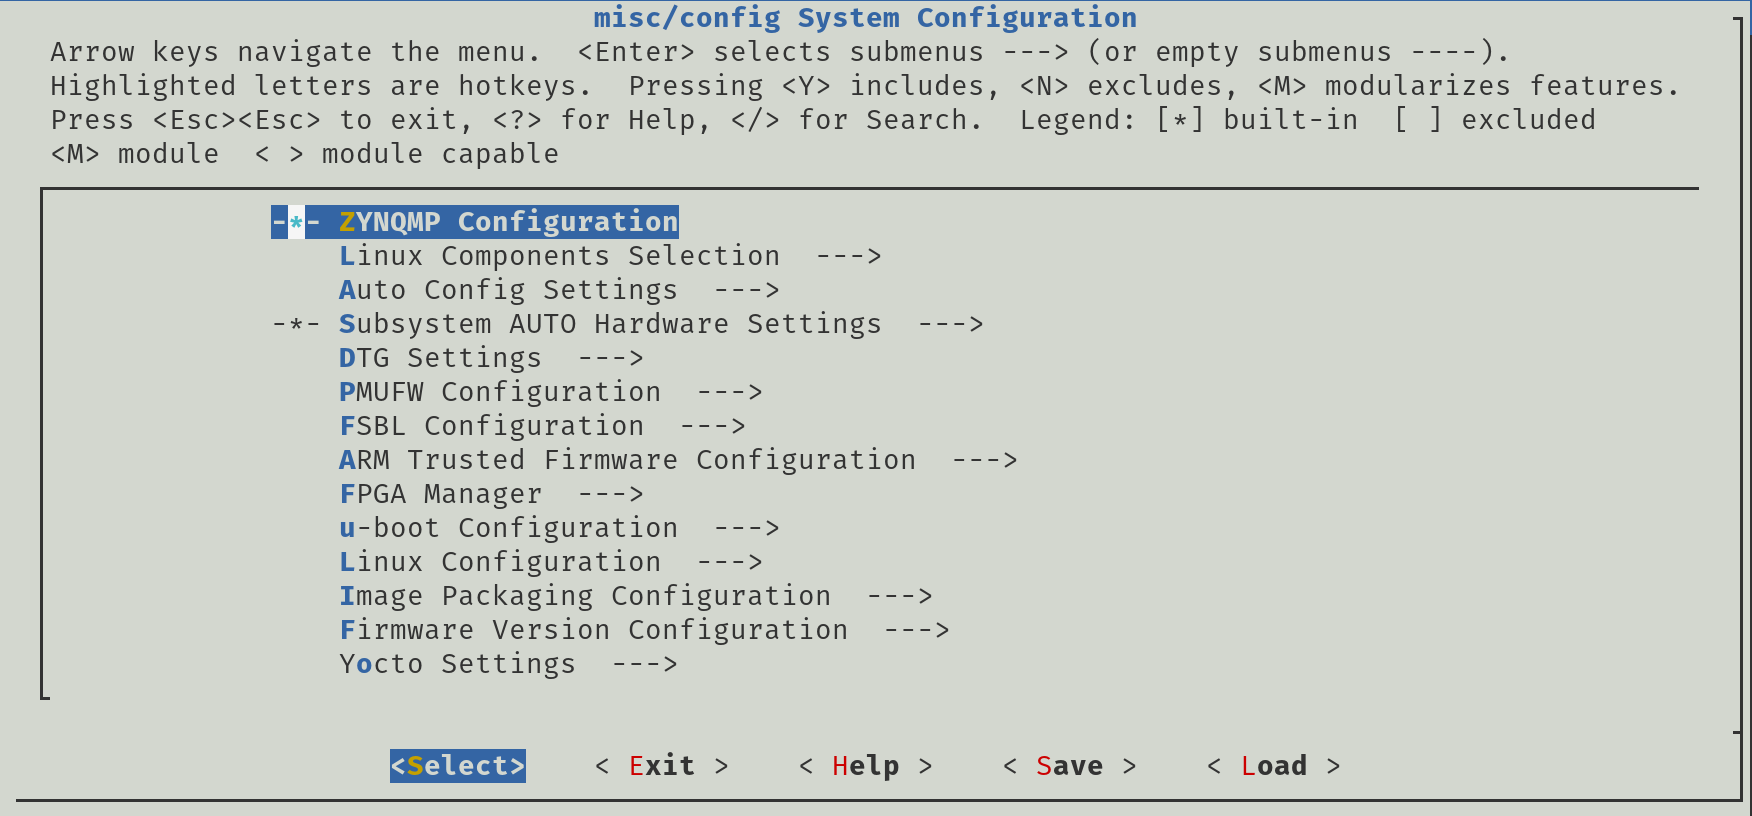
\includegraphics[width=1\textwidth]{./images/petalinux_config.jpg}
	\end{center}
	\vspace{-5pt}
	\caption[Menuconfig Startbildschirm des PetaLinux-Projekts]{Menuconfig Startbildschirm des PetaLinux-Projekts} % Eckige Klammer (optional): Caption-Text in Abbildungsverzeichnis
	\label{fig:menuconfig}
	\vspace{-5pt}
\end{figure}

Die Abbildung ~\ref{fig:menuconfig} zeigt der Menuconfig Startbildschirm, der erscheint, nachdem der Befehl \textbf{petalinux-config} die nach dem Befehl \textbf{petalinux-create} erzeugten Kconfig-Dateien analysiert hat. Diese Menuconfig ist eigentlich ausreichend, um das gesamte Projekt zu konfigurieren, aber man kann jedoch auch individuelle Konfigurationen für Boot-Komponenten mit einer ähnlichen Menuconfig-Schnittstelle vornehmen. Diese Individuelle Komponenten Konfigurationen sind nämlich wichtig wenn man  komplexe Konfigurationen vornehmen soll. So gibt es eine Menuconfig für den Kernel, das U-boot, das Rootfs ...\\
Damit unser MCP251xfd CAN-Controller erkannt und in Betrieb genommen werden kann, sollte man z.B. das Kernel-Menüocnfig verwenden, um den Treiber zu integrieren. Absichtlich wurde Petalinux 2021 verwendet, da für den Chip ein Treiber vorhanden ist. 

\begin{figure}[H]
	\begin{center}		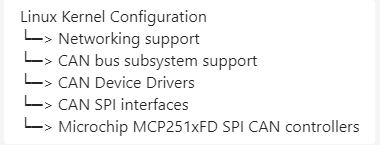
\includegraphics[width=0.7\textwidth]{./images/mcp_driver_pfard.jpg}
	\end{center}
	\vspace{-5pt}
	\caption[Pfard zur mcp251xfd Treiber]{Pfard zur mcp251xfd Treiber} % Eckige Klammer (optional): Caption-Text in Abbildungsverzeichnis
	\label{fig:mcp:treiber:pfard}
	\vspace{-5pt}
\end{figure}

Der oben gezeigte Pfad führt uns zum Kernel-Fenster, wo man den Treiber für den MCP251xFD aktivieren oder deaktivieren kann. Die Abbildung ~\ref{fig:mcp:treiber} zeigt alle CAN-Controller mit SPI-Schnittstelle, die uns der Kernel 5.10 bietet. Hier können sie auch als Modul aktiviert werden, so dass der Treiber nach dem Bootvorgang geladen oder entladen werden kann. Dies wurde in dieser Arbeit genutzt, um zu überprüfen, ob der Treiber den Mikrochip korrekt initialisiert hat.

\begin{figure}[H]
	\begin{center}		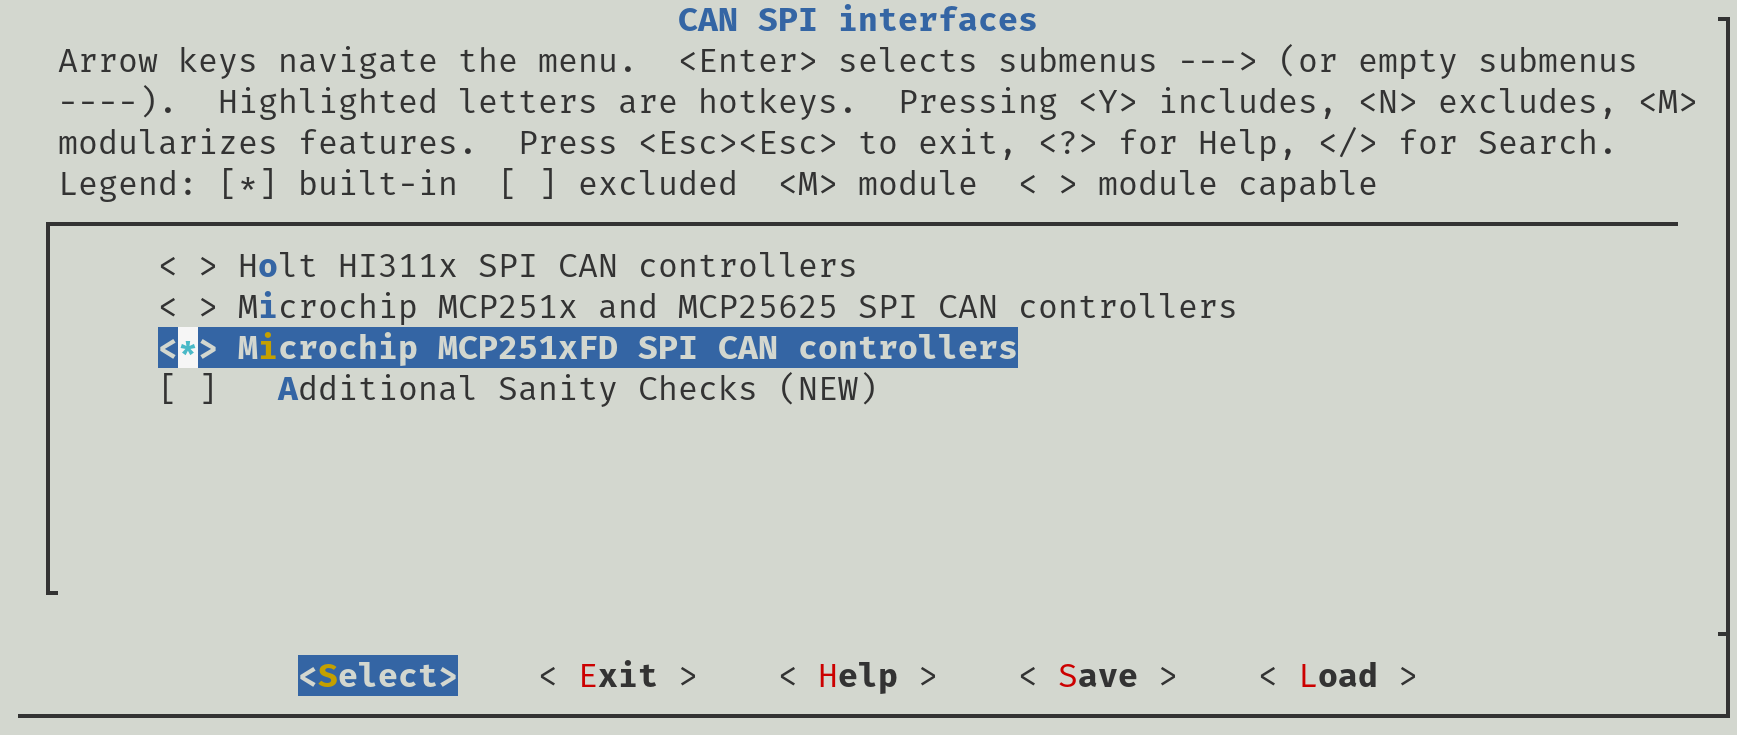
\includegraphics[width=1\textwidth]{./images/mcp_treiber.jpg}
	\end{center}
	\vspace{-5pt}
	\caption[Konfig Fenster mcp251xfd Treiber]{Konfig Fenster mcp251xfd Treiber} % Eckige Klammer (optional): Caption-Text in Abbildungsverzeichnis
	\label{fig:mcp:treiber}
	\vspace{-5pt}
\end{figure}

\subsection{Device-Tree Eintrag für den MCP251XFD CAN-Controller }
\begin{figure}[H]
	\begin{center}		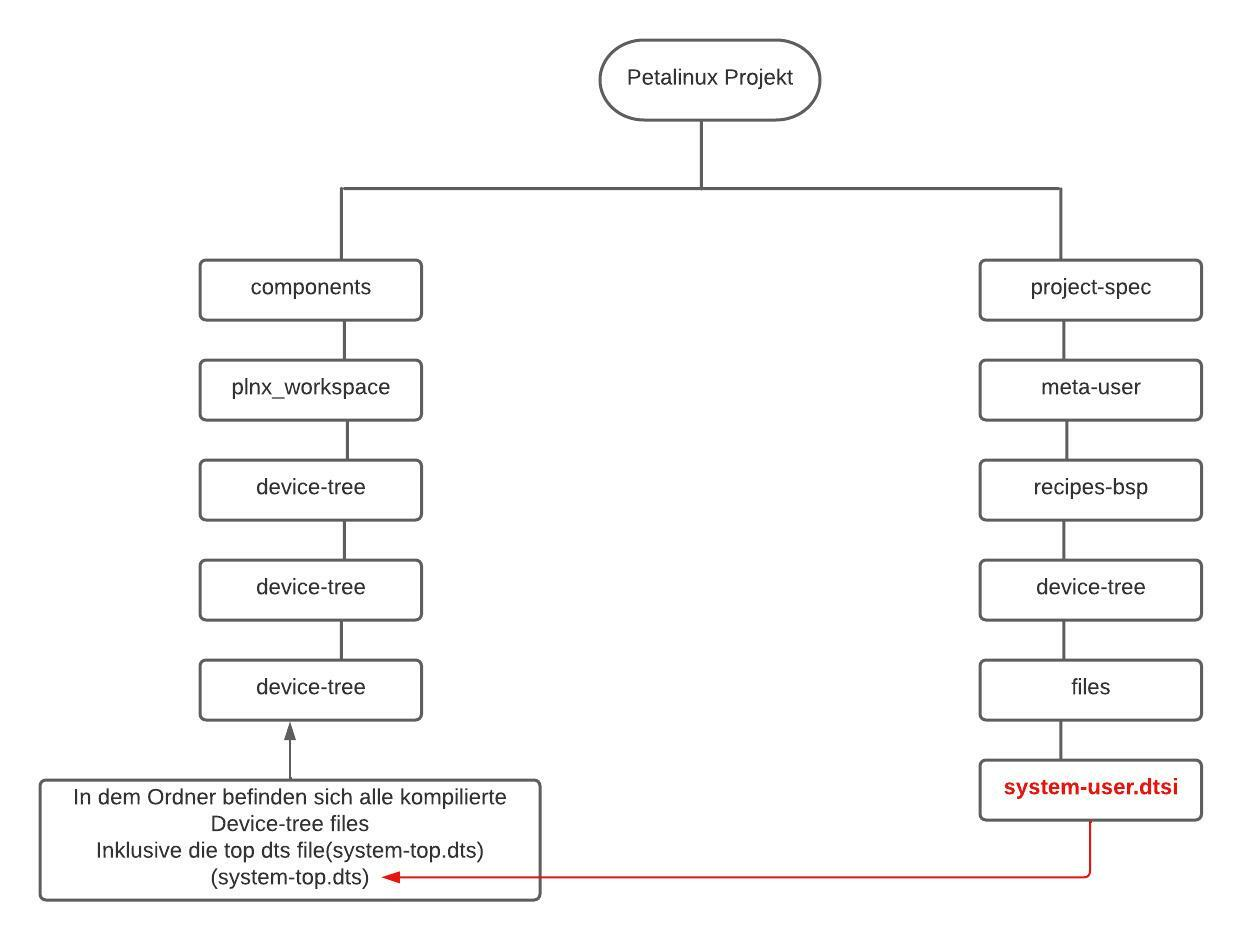
\includegraphics[width=1\textwidth]{./images/device-tree-diagram.jpg}
	\end{center}
	\vspace{-5pt}
	\caption[Device-tree Projekt Struktur]{Device-tree Projekt Struktur} % Eckige Klammer (optional): Caption-Text in Abbildungsverzeichnis
	\label{fig:deviceTree:struktur}
	\vspace{-5pt}
\end{figure}

Damit unser Mikrochip nach dem Bootvorgang in Betrieb genommen werden kann, müssen dem Kernel Informationen (wie z.B. der Name des Hardwaretreibers, die Taktfrequenz oder der Interrupt-Pin...) übergeben werden, damit die Hardware während des Bootvorgangs initialisiert wird. Daher wird in Petalinux empfohlen, die Datei \textbf{system-user.dtsi} zum Hinzufügen, Löschen oder Ändern eines Gerätebaumknotens zu verwenden. Diese Datei befindet sich in \textbf{<project>/project spec/meta-user/recipes-bsp/device-tree/files/}. Sie wird an das Ende der Datei system-top.dts gestellt wie im Listing ~\ref{lst:device:tree:top} dargestellt, so dass sie eine höhere Priorität erhält, und wird somit zuerst kompiliert.

%\newpage

\begin{lstlisting}[backgroundcolor = \color{lightgray},basicstyle=\scriptsize\ttfamily,caption={Inhalt der system-top.dts Datei},label=lst:device:tree:top,language=bash,framexleftmargin = 2em]
/dts-v1/;
#include "zynqmp.dtsi"
#include "zynqmp-clk-ccf.dtsi"
#include "zcu106-reva.dtsi"
#include "pcw.dtsi"
/ {
	chosen {
		bootargs = "earlycon";
		stdout-path = "serial0:115200n8";
	};
	aliases {
		ethernet0 = &gem3;
		i2c0 = &i2c0;
		i2c1 = &i2c1;
		serial0 = &uart0;
		serial1 = &uart1;
		spi0 = &qspi;
		spi1 = &spi0;
	};
	memory {
		device_type = "memory";
		reg = <0x0 0x0 0x0 0x7ff00000>, <0x00000008 0x00000000 0x0 0x80000000>;
	};
};
#include "system-user.dtsi"	
\end{lstlisting}

Das Petalinux-Projekt wurde mit einer von Vivado exportierten Hardwarebeschreibungsdatei (HDF-Datei) konfiguriert, in der bestimmte Vorkonfigurationen bereits vorgenommen wurden. Beispielsweise die Konfiguration der Pins, des gpio-Controllers, des SPI-Controllers usw. 

\begin{figure}[H]
	\begin{center}		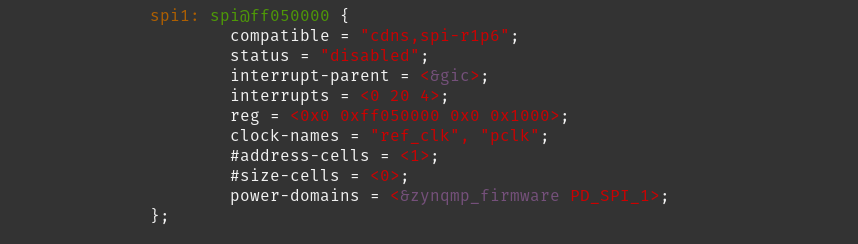
\includegraphics[width=1\textwidth]{./images/xilinx_spi_controller.jpg}
	\end{center}
	\vspace{-5pt}
	\caption[Xilinx SPI-Controller]{Xilinx SPI-Controller} % Eckige Klammer (optional): Caption-Text in Abbildungsverzeichnis
	\label{fig:deviceTree:spi:controller}
	\vspace{-5pt}
\end{figure}

Der Code, der in Abbildung ~\ref{fig:deviceTree:spi:controller} zu sehen ist. beschreibt den im Vivado implementierten Xilinx-SPI-Controller, an den unser CAN-Controller angeschlossen werden soll. im \textbf{reg} ist die Basisadresse und der Adressbereich, in dem der SPI-Controller betrieben wird. \\
Der Code, der in den aktuellen Device-tree für den CAN-Controller eingefügt werden muss, ist der unten stehende.
\begin{lstlisting}[backgroundcolor = \color{lightgray},basicstyle=\scriptsize\ttfamily,caption={Device-tree Eintrag für den mcp251xfd CAN-Controller},label=lst:device:tree:mcp,language=bash,framexleftmargin = 2em]
	
	/include/ "system-conf.dtsi"
	/ {
		can0_osc: can0_osc {
			compatible = "fixed-clock";
			#clock-cells = <0>;
			clock-frequency = <20000000>;
		};
	};
	
	&spi0 {
		#address-cells = <1>;
		#size-cells = <0>;
		can@0 {
			compatible = "microchip,mcp251xfd";
			reg = <0>;
			clocks = <&can0_osc>;
			pinctrl-names = "default";
			//pinctrl-0 = <&can0_pins>;
			interrupts-extended = <&gpio 78 8>;
			spi-max-frequency = <8333333>;
			microchip,rx-int-gpios = <&gpio 79 1>;
		};
	};
\end{lstlisting}

wichtige Information dazu wurde in den folgende Tabelle zusammengefasst. 

\begin{tabular}{lp{11cm}}
	\toprule
	\textbf{Funktion} &\textbf{Beschreibung}\\
	\midrule
	\textit{compatible} & wird verwendet, um zu entscheiden, wie das Gerät ausgeführt werden soll und das Gerät mit dem Treiber zu verbinden. Er enthält eine Zeichenkette in der Form <Hersteller>,<Modell>. In unseren Fall handelt es sich um ein microchip herstellte mcp251xfd.\\
	\textit{reg = <0>} & dem CAN-Controller wird eine eindeutige ID zugewiesen, der hat  also keine Adresse Bereich. \\
	\textit{clocks} & Der interne Taktgenerator im Controller wird hier beschrieben. Der kann 40, 20 oder 4 MHz generieren. Hier wurde er aber auf 20 MHz eingestellt.\\
	\textit{interrupts-extended} & Hier werden die vom Gerät erzeugten Interrupts aufgelistet. Es wird auch spezifiziert an welchem GPIO-Pin diese Interrupts empfangen werden.\\
	\textit{spi-max-frequency} & steht für die maximale SPI-Taktfrequenz des Geräts. Diese wurde auf 8,33 MHz gesetzt, da für eine gute Kommunikation mit dem SPI-Master die SPI-Taktfrequenz die Hälfte oder weniger des Takts betragen sollte. \\
	\bottomrule
\end{tabular}
\subsection{Rezepte zur Kompilierung der Software Modulen}
\subsection{Bauen des Systems}

